% ICCIT 2026 submission, draft 3. IEEE conference template, A4 (ICCIT requires the A4 template).
% DOUBLE-BLIND: no author names, affiliations, addresses, or emails anywhere.
% FRAMING: one investigation, four levers. See Defense/ICCIT/DRAFT3_PLAN.md.
% Every number here is verified in Defense/ICCIT/AUDIT_2026-08-21.md.
% Build: pdflatex main && bibtex main && pdflatex main && pdflatex main
\documentclass[conference,a4paper]{IEEEtran}
\IEEEoverridecommandlockouts
\usepackage{cite}
\usepackage{amsmath,amssymb,amsfonts}
\usepackage{graphicx}
\usepackage{textcomp}
\usepackage{xcolor}

\begin{document}

\title{MSA-YOLO: Attention, Scale, and Supervision\\
for Tiny-Human Detection in Aerial\\
Search-and-Rescue Imagery}

% Double-blind submission: author block anonymized per ICCIT 2026 guidelines.
\author{\IEEEauthorblockN{Anonymous Submission}
\IEEEauthorblockA{\textit{Paper ID assigned by CMT}}}

\maketitle

\begin{abstract}
A person photographed from a drone over a disaster site may span fewer than ten
pixels, which is below the resolving limit of a standard detection head. Work on
this regime adds attention modules, higher-resolution detection scales, sliced
inference or state-space blocks, usually one at a time and on different data, so
the relative worth of each is unknown. This paper asks where recall of
sub-8-pixel people actually comes from, and measures four candidate answers on
one detector under one protocol. Attention buys 0.3 points and arrives at a
negative parameter cost. A stride-4 detection scale buys a further 1.1 points
and is the strongest network-side option; the two together define MSA-YOLO,
which reaches 0.853 AP50 with 19.6 million parameters, second among published
C2A results to a detector three times its size. A bidirectional state-space neck
buys nothing for 2.4 million parameters and 2.8 times the latency. A tiny-aware
change to label assignment, which touches training only and adds no inference
cost, buys 2.08 points, more than any change to the network, with a bootstrap
interval that excludes zero and a positive effect across three seeds. The same
detector was then run on real drone and disaster footage collected for this
study. Zero-shot it reaches 0.335 and 0.133 AP50; 248 labeled real frames raise
those to 0.795 and 0.411 while the synthetic benchmark holds at 0.837. Below 8
pixels on real frames, recall is zero.
\end{abstract}

\begin{IEEEkeywords}
tiny object detection, aerial human detection, search and rescue, attention,
multi-scale detection, label assignment, UAV imagery
\end{IEEEkeywords}

\section{Introduction}
When an earthquake or a flood strikes, the first hours decide how many people
are found alive. A drone can sweep a disaster site far faster than a ground
team, but the imagery it returns is punishing to search by eye: a person seen
from altitude spans a few dozen pixels at best, and one sortie produces
thousands of frames. Automating that search is a practical need rather than a
convenience.

The difficulty is geometric. A one-stage detector predicts boxes on a grid whose
cell covers a stride-sized region of the input, so at the finest standard scale,
stride 8, a twelve-pixel person spans about one and a half cells, and a detector
cannot localize what falls inside a fraction of one cell.
In the C2A disaster benchmark used here~\cite{nihal2024c2a}, about 47\% of
annotated people are smaller than ten pixels.

\begin{figure}[t]
\centerline{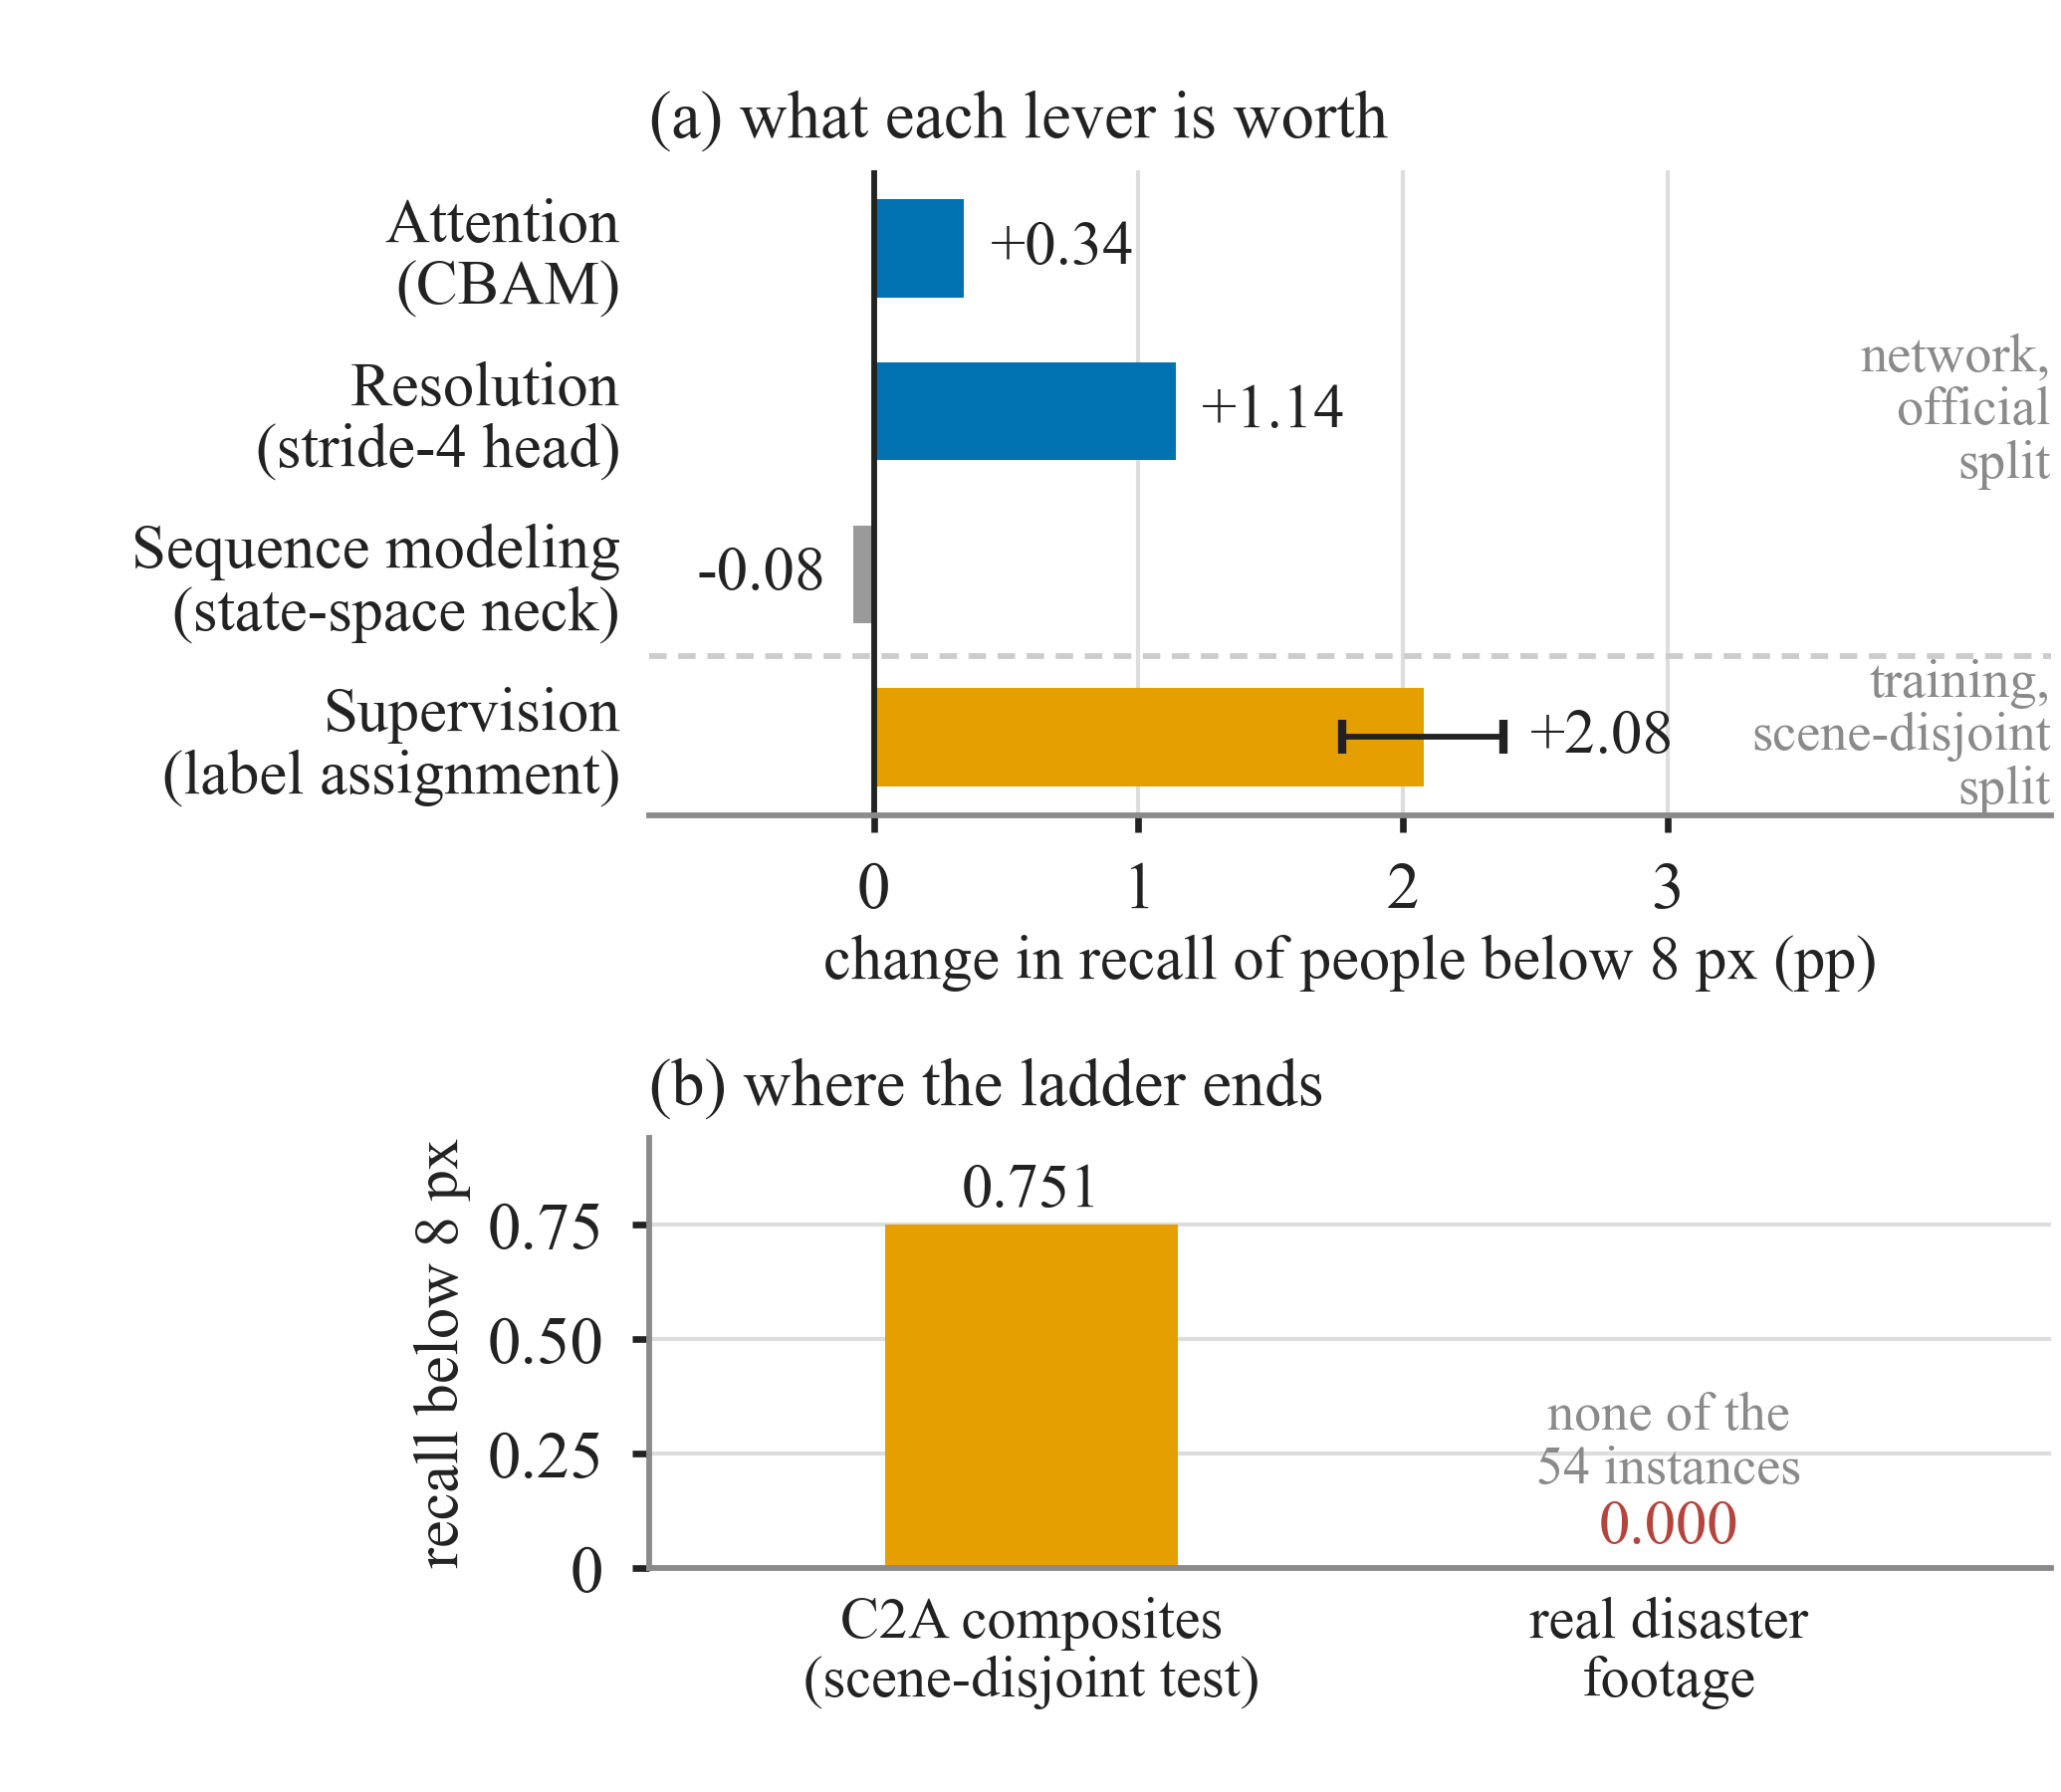
\includegraphics[width=\columnwidth]{figures/fig_answer.png}}
\caption{Where recall of sub-8-pixel people comes from. (a) The effect of each
lever, measured as the change from the configuration directly above it inside
the same training protocol. The three network changes were measured on the
official C2A split and the supervision change on a scene-disjoint re-split of
the same data, so each bar is an effect within its own protocol and the four do
not share an absolute level. The whisker is the paired image-level bootstrap 95\%
interval on the supervision delta, which is positive in all three seeds
retrained, mean 1.62 points. (b) Recall below 8 px for the strongest model on
each source of imagery: 0.751 on C2A composites against none of the 54
sub-8-pixel people present in real disaster frames.}
\label{fig:answer}
\end{figure}

Remedies for this regime exist and are individually plausible. Higher-resolution
detection scales~\cite{zhu2021tphyolov5}, feature
attention~\cite{woo2018cbam,wang2020eca}, sliced
inference~\cite{akyon2022sahi} and state-space
necks~\cite{gu2023mamba,wang2025mambayolo} have all been proposed. They are
usually reported one at a time, on different aerial data, and without a shared
training protocol, so anyone building a rescue detector today has to guess which
addition earns its cost. A fourth family of methods changes neither the network
nor the input but the training step that decides which predictions are
supervised~\cite{wang2021nwd,xu2022rfla,shi2024simd}, and it is rarely compared
against the architectural options at all.

\begin{figure*}[t]
\centerline{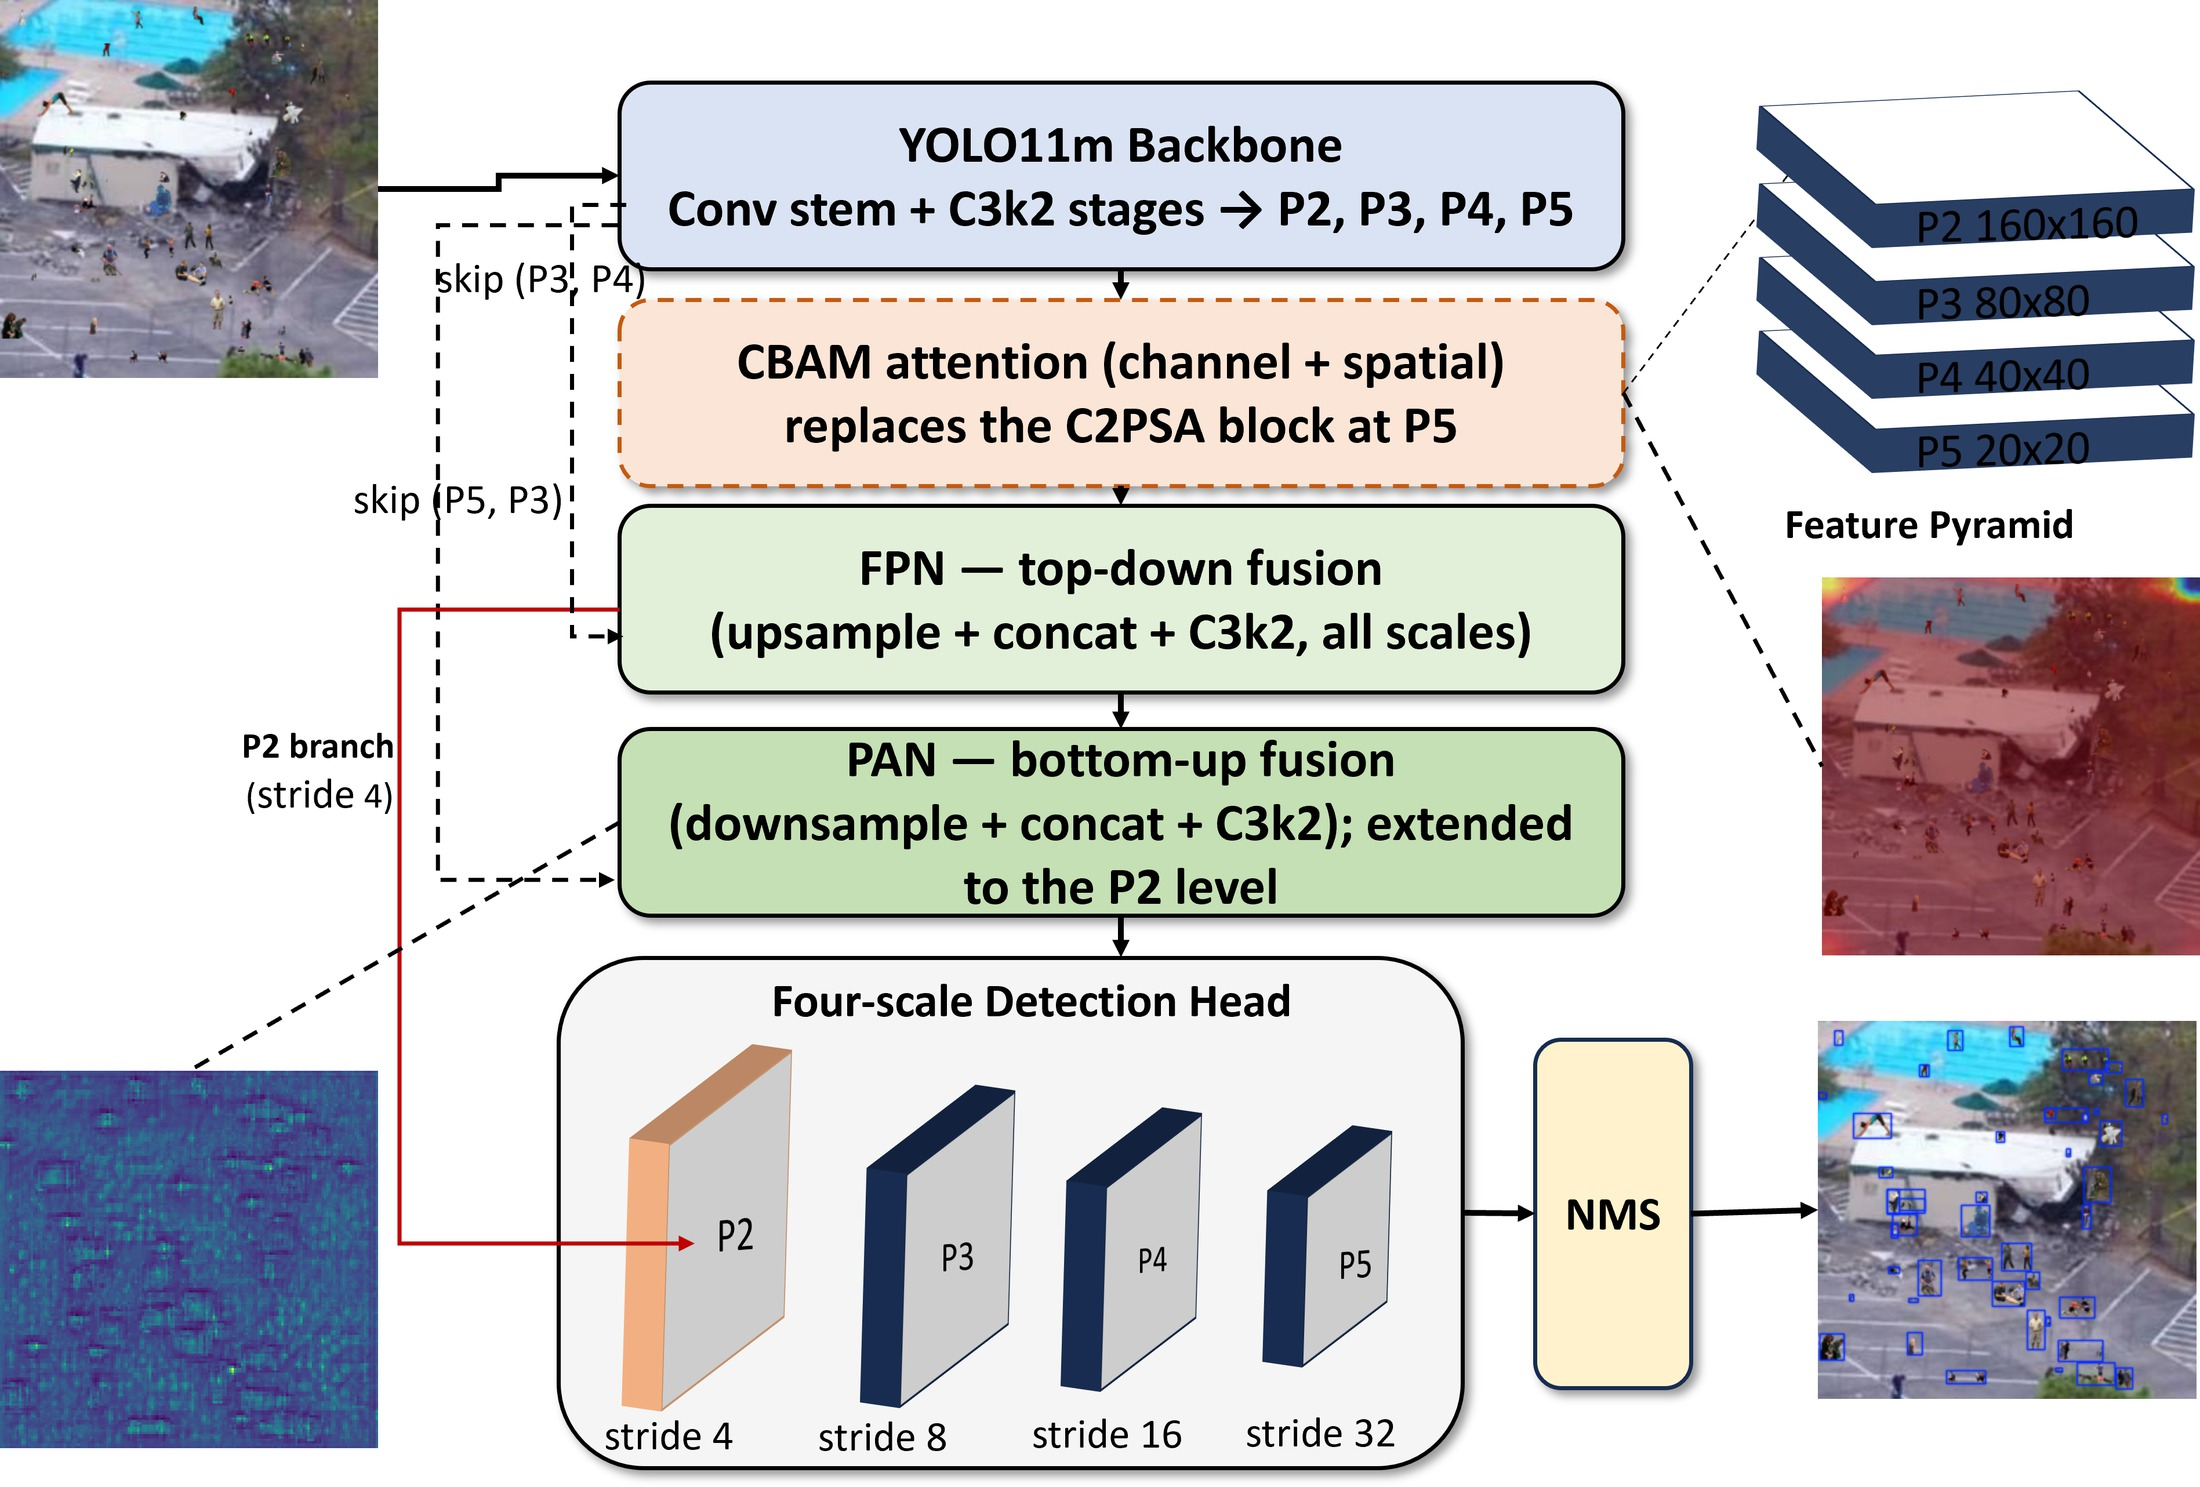
\includegraphics[width=0.94\textwidth]{figures/fig_arch.jpg}}
\caption{MSA-YOLO on a C2A scene. The backbone produces features at five
resolutions; CBAM (orange) replaces the terminal self-attention block and
re-weights the deepest features; the neck fuses scales and is carried one level
further than the standard design to produce a stride-4 branch, so the head
decodes at strides 4, 8, 16 and 32. The insets are the model's own signals on
this scene: input, attention response, stride-4 feature response, and final
detections. Note that the stride-4 map responds at the smallest scattered
figures, which the stride-8 level summarizes into single cells.}
\label{fig:arch}
\end{figure*}

This paper treats those options as one question. We ask where recall of
sub-8-pixel people comes from, and we answer it by putting four levers on a
single detector and measuring each under a fixed protocol: channel-and-spatial
attention, a stride-4 detection scale, a bidirectional state-space neck, and the
overlap measure the label assigner uses. Fig.~\ref{fig:answer} gives the result
in advance. The two levers that pay for themselves in the network define
MSA-YOLO, an enhancement of YOLO11m~\cite{jocher2024yolo11} that modifies the
baseline in exactly two places. The lever that pays most, however, is not in the
network at all. We then take the same detector to real drone and disaster
footage collected and annotated for this study, because a model trained on
composited scenes has never been asked what it does on real ones, and there the
ladder runs out: below 8 px on real frames nothing is recovered.

The contributions are the following.
\begin{itemize}
\item A single-protocol comparison of four levers for sub-8-pixel recall, with
each effect attributed separately, showing that the assignment of supervision
outweighs every change made to the network.
\item MSA-YOLO, the strongest network-side configuration found, at 0.853 AP50
and 19.6 million parameters, second only to a detector three times its size
among published results on C2A, together with a documented negative result for
a state-space neck that cost 2.4 million parameters and 2.8 times the latency.
\item A tiny-aware label-assignment blend that adds 2.08 points of sub-8-pixel
recall at no parameter or inference cost, with a bootstrap interval excluding
zero and a positive effect in all three seeds tested.
\item A real-footage study on our own drone, campus and disaster imagery that
quantifies the synthetic-to-real gap, shows what 248 labeled frames buy, and
reports where that budget stops paying.
\end{itemize}

\section{Related Work}
Object detection divides into two-stage detectors in the R-CNN
line~\cite{ren2015fasterrcnn,cai2018cascade}, one-stage detectors such as
SSD~\cite{liu2016ssd}, RetinaNet~\cite{lin2017focal} and the YOLO
family~\cite{redmon2016yolo,wang2024yolov9,jocher2024yolo11}, and transformer
designs such as DETR~\cite{carion2020detr} and RT-DETR~\cite{zhao2024rtdetr}. We
work inside the one-stage YOLO family because its speed and small model size
suit airborne deployment.

Detecting very small objects is a distinct problem~\cite{cheng2023smallobject},
and the literature attacks it in four places. It adds resolution, where feature
pyramids~\cite{lin2017fpn} and a stride-4 head extend detection to targets a few
pixels wide~\cite{zhu2021tphyolov5}. It re-weights features, using channel
attention~\cite{wang2020eca} or combined channel-and-spatial
attention~\cite{woo2018cbam}. It works at inference time, slicing the image into
overlapping crops~\cite{akyon2022sahi}. And it changes the training step that
selects positive samples, on the observation that intersection over union
collapses for tiny boxes: Wang et al.~\cite{wang2021nwd} replaced it with a
normalized Wasserstein distance, RFLA~\cite{xu2022rfla} built assignment on a
receptive-field prior, and SimD~\cite{shi2024simd} learned an adaptive
similarity. Modern YOLO versions assign samples with the task-aligned assigner
of TOOD~\cite{feng2021tood}, which still scores localization with the IoU
family, and none of the tiny-object assignment work above has been placed inside
it for aerial person detection. Section~\ref{sec:assign} takes that opening, and
Section~\ref{sec:where} measures it against the other three families on the same
detector, which to our knowledge has not been done.

Real search-and-rescue collections such as SARD~\cite{sambolek2021sard} and
HERIDAL~\cite{bozic2019heridal} hold only a few thousand frames.
C2A~\cite{nihal2024c2a} instead composites segmented human figures onto real
disaster backgrounds~\cite{kyrkou2020aider}, giving 10{,}215 images and roughly
360{,}000 instances. Results on such data are almost always in-domain, which
leaves transfer untested. Work on domain
randomization~\cite{tobin2017domainrand} and on fine-tuning synthetic-trained
models with a little real data~\cite{tremblay2018synthetic} suggests the recipe
of Section~\ref{sec:real}.

\section{Four Levers on One Detector}
The four levers act in different places, which is what makes the comparison
possible: two change the network, one changes the neck only, and one changes
nothing that runs at inference time. All four sit on the same YOLO11m baseline,
in which an aerial image is letterbox-resized to $640 \times 640$, passed
through the backbone, fused across scales by a path-aggregation neck, and
decoded by a multi-scale head before non-maximum suppression.

\subsection{Attention and Scale: MSA-YOLO}
The first lever replaces the self-attention block that follows the
spatial-pyramid-pooling stage with a convolutional block attention
module~\cite{woo2018cbam}, which applies channel attention and then spatial
attention with a reduction ratio of 16 and a $7 \times 7$ spatial kernel. The
module is lighter than the block it replaces, so whatever it earns is earned at
a negative parameter cost.

The second lever adds resolution, for the reason drawn in
Fig.~\ref{fig:stride}. The neck's top-down pass continues one level below the
standard design: the fused stride-8 feature is upsampled, concatenated with the
backbone feature at stride 4, and fused into a $160 \times 160$ map that a
fourth detection branch reads. The existing three levels are untouched, which
keeps the addition attributable. These two changes together are MSA-YOLO,
drawn in Fig.~\ref{fig:arch}.

\begin{figure}[t]
\centerline{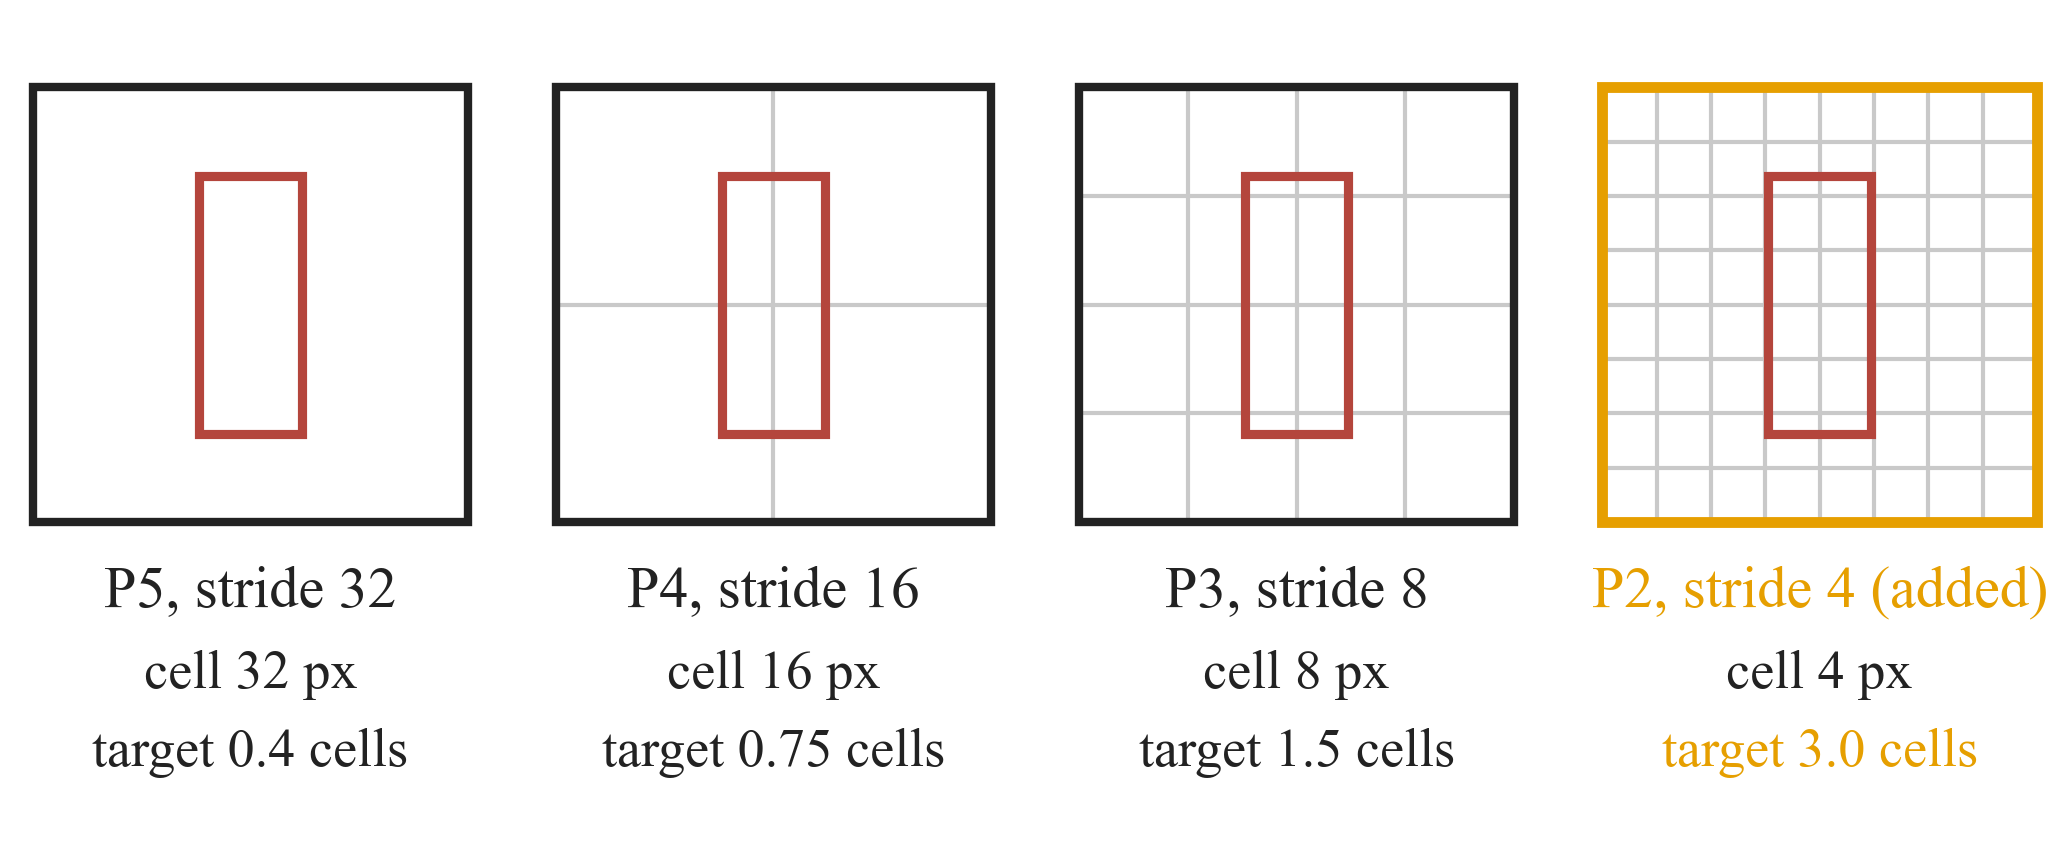
\includegraphics[width=\columnwidth]{figures/fig_stride.png}}
\caption{Why a stride-4 scale is added. Each panel is the same 32 by 32 px patch
of a 640 px input, holding one identical target box. A detection cell covers a
stride-sized region, so a target of side $s$ spans $s/d$ cells at stride $d$: the
box here falls inside a fraction of one cell at the two coarsest levels and
covers about 1.5 cells at stride 8, the finest standard level. Stride 4 is the
first level that gives it about three cells, which is enough spatial support to
regress an offset from.}
\label{fig:stride}
\end{figure}

\subsection{A State-Space Neck}
The third lever tests the claim that state-space blocks improve feature
aggregation. A variant replaces the bottleneck at six neck layers with a block
performing bidirectional local-window selective scans, inserted so that the
backbone and the head are unchanged. Its scan diagnostics confirm the module was
active, with a mean forward-to-reverse cosine distance of 0.836.

\subsection{Tiny-Aware Label Assignment}
\label{sec:assign}
The fourth lever leaves the network alone. Modern YOLO versions select positive
samples with a task-aligned assigner that scores each candidate by
$t = s^{p} u^{q}$, where $s$ is a classification score and $u$ a localization
overlap measured with the complete IoU. That measurement is the weak point at
this scale: for a person a few pixels wide a one-pixel offset can drive the IoU
to zero, so candidates for the smallest targets are ranked with almost no signal
and those people are trained on poorly chosen samples. The network can be made
as sharp as one likes and this will still be true.

We keep the assigner and replace only its overlap term. For a ground-truth box
$g$ and a candidate $b$ with centers, widths and heights $(c_x, c_y, w, h)$, the
squared 2-Wasserstein distance between Gaussians fitted to the boxes is
\begin{equation}
  W_2^2(g,b) = (c_{x}^{g}\!-\!c_{x}^{b})^2 + (c_{y}^{g}\!-\!c_{y}^{b})^2
    + \tfrac{1}{4}\big[(w^{g}\!-\!w^{b})^2 + (h^{g}\!-\!h^{b})^2\big],
\end{equation}
and the normalized Wasserstein similarity~\cite{wang2021nwd} maps it into
$(0,1]$ as $S(g,b) = \exp(-W_2(g,b)/C)$ with $C$ set to the median person size
of the dataset in pixels, here 12.8. Unlike the IoU, this similarity stays
informative for disjoint tiny boxes: a near miss scores above a distant one even
when both overlap nothing. The overlap the assigner consumes becomes
\begin{equation}
  u = (1-\gamma)\,\mathrm{CIoU}(g,b) + \gamma\, S(g,b),
  \label{eq:blend}
\end{equation}
where $\gamma$ sets how far assignment trusts the scale-tolerant similarity, and
$\gamma = 0$ recovers the unmodified assigner. The change affects training only.
It adds no parameters and no inference cost, and it is distinct from placing the
same distance inside the regression loss, which we also tried without success.

\section{Experimental Setup}
All training and evaluation ran on one workstation with an NVIDIA RTX 4070 Ti
SUPER (16 GB), an Intel Core i7-14700K and 128 GB of RAM, using Python 3.11,
PyTorch 2.12 with CUDA 12.6, and Ultralytics 8.4.56. Every configuration used
AdamW at a base learning rate of 0.001 with a cosine schedule, up to 300 epochs
with early stopping on fitness and on $F_2$, mixed precision, and seed 0. The
optimizer was pinned because the framework default diverged on the four-scale
head. Batch size was 16, reduced to 8 physical with gradient accumulation for
the stride-4 models, whose extra scale raises activation memory.

C2A~\cite{nihal2024c2a} provides 10{,}215 images with roughly 360{,}000 person
instances across collapsed-building, fire, flood and traffic scenes. Two
protocols are used, and they are never mixed within a table. The \emph{official}
split (6{,}129 training, 2{,}043 validation, 2{,}043 test images) carries the
network comparison, because published results on this benchmark use it. An audit
of scene identifiers found that 98\% of official test scenes also appear in
training, since several composited images share one background, so we also built
a \emph{scene-disjoint} re-split (6{,}135 / 2{,}040 / 2{,}040) in which all
images of a scene fall on one side. Retraining the recommended model there costs
1.6 points of AP50 and 1.2 points of sub-8-pixel recall, so the leakage inflates
the official protocol modestly and changes no conclusion. The assignment and
real-footage experiments use the clean split.

Because a missed person costs more than a false alarm, the primary operating
metric is the recall-weighted $F_2$ score. We also report AP50, COCO average
precision, average recall at 100 detections, recall in the size bands very-tiny
(under 8 px), tiny (8 to 16 px), small (16 to 32 px) and medium (32 to 96 px)
measured as the square root of box area, and end-to-end latency including
preprocessing and non-maximum suppression. Where two models are compared on one
set, a paired image-level bootstrap over 1{,}000 resamples gives a 95\%
confidence interval and a two-sided $p$-value.

\section{Where Sub-8-Pixel Recall Comes From}
\label{sec:where}

\subsection{The Three Network Levers}
Table~\ref{tab:abl} introduces one network change at a time on the official C2A
test set. Aggregate average precision is saturated, with all four models inside
0.002 AP of one another, which is expected when annotation noise dominates at
strict IoU thresholds for boxes this small. The differences appear where the
task lives. The stride-4 scale is the effective change: on top of attention it
lifts AP50 from 0.847 to 0.853, average recall from 0.692 to 0.703, sub-8-pixel
recall from 0.746 to 0.757, and operational $F_2$ from 0.841 to 0.844, for about
half a million
parameters and one millisecond. The attention substitution is close to free. It
removes roughly one million parameters relative to the baseline, gives the
lowest latency of the four, and improves every accuracy column slightly. The
state-space neck is the outlier in the wrong direction, adding 2.4 million
parameters and taking latency from 14.6 to 41.1 ms while matching, not beating,
the configuration below it. On this evidence MSA-YOLO is the attention plus
stride-4 configuration, and the state-space neck is not carried forward.

\begin{table}[htbp]
\caption{Additive Ablation on the Official C2A Test Split. Par.: parameters in
millions; GF: GFLOPs; AR: average recall at 100 detections; VT: recall below
8 px; ms: end-to-end latency.}
\label{tab:abl}
\begin{center}
\footnotesize
\setlength{\tabcolsep}{3pt}
\begin{tabular}{|l|c|c|c|c|c|c|c|}
\hline
\textbf{Configuration} & \textbf{Par.} & \textbf{GF} & \textbf{AP50} & \textbf{AP} & \textbf{AR} & \textbf{VT} & \textbf{ms} \\
\hline
YOLO11m & 20.03 & 67.7 & 0.843 & 0.615 & 0.691 & 0.743 & 13.7 \\
\hline
+ CBAM & 19.08 & 66.9 & 0.847 & 0.616 & 0.692 & 0.746 & 13.5 \\
\hline
+ CBAM + P2 & 19.57 & 86.7 & \textbf{0.853} & 0.615 & 0.703 & \textbf{0.757} & 14.6 \\
\hline
+ SSM neck & 22.01 & 98.4 & 0.852 & 0.614 & 0.704 & 0.757 & 41.1 \\
\hline
\end{tabular}
\end{center}
\end{table}

Recall by size explains the flat aggregate. The stride-4 scale trades a little
accuracy on larger targets for its gain at the bottom: tiny-band recall moves
from 0.873 to 0.865 and small-band recall from 0.895 to 0.886, while the medium
band falls from 0.912 to 0.808. That last figure looks severe but rests on 317
of roughly 72{,}500 test instances, so it is noisy. The net effect is a model
that is better where the dataset lives, since 99.6\% of instances are below
32 px. Calibration is stable across the chain, with expected calibration error
between 0.020 and 0.023, so a reported confidence can be read as an empirical
precision. Two inference-time procedures were also measured on the recommended
model without retraining: slicing~\cite{akyon2022sahi} at a 256-pixel tile
raises sub-8-pixel recall from 0.758 to 0.788 at 162 ms per image against 15 ms,
while test-time augmentation at 1280-pixel input reaches 0.850 recall and 0.854
$F_2$ at 60 ms. Both are operating modes that buy recall with latency rather
than levers on the model.

\subsection{The Supervision Lever}
The assignment blend of Equation~\eqref{eq:blend} was evaluated on the
scene-disjoint split, so its numbers are not comparable to Table~\ref{tab:abl}
and are reported as a matched difference. Fifty-epoch pilots swept $\gamma$ and
found a monotonic trade: sub-8-pixel recall rises from 0.693 at $\gamma = 0$ to
0.712 at $\gamma = 0.5$ and 0.729 at $\gamma = 1$, while small-object average
precision falls from 0.560 to 0.553 and then to 0.505. The half blend takes about
half of the available recall gain for an eighth of the precision cost, and was
carried forward.

Table~\ref{tab:assign} reports the decisive test, a matched pair at the full
protocol in which two runs share launcher, initialization, split and schedule
and differ only in $\gamma$. The blend raises sub-8-pixel recall from 0.730 to
0.751, a gain of 2.08 points whose 95\% bootstrap interval $[1.77, 2.38]$
excludes zero at $p < 0.001$, and it holds the overall operating score while
paying about one point in each of the two bands above. Retraining both models at
two further seeds reproduces the effect: counting the pair above as the first,
the three seeds give 2.08, 1.66 and 1.11 points, a mean of 1.62 with a standard
deviation of 0.49, positive in every seed. One sub-claim did not
survive that replication: a two-point small-object average-precision gain seen at
seed 0 averaged to noise across seeds and is therefore not claimed.

The size of this effect is the paper's main observation. A change that adds no
parameters, no FLOPs and no latency moves recall at the hardest size band by more
than the three network changes moved it between them, 2.08 points against 1.40.
The two figures come from different protocols, so this compares effect sizes and
not levels, but the ordering is not close. For targets a few pixels wide the
network is not the binding constraint; which predictions get supervised is.

\begin{table}[htbp]
\caption{Matched Pair Differing Only in the Assignment Blend, Scene-Disjoint
Split. Changes are in points; the interval is a paired image-level bootstrap.}
\label{tab:assign}
\begin{center}
\small
\setlength{\tabcolsep}{4pt}
\begin{tabular}{|l|c|c|c|c|}
\hline
\textbf{Metric} & $\gamma = 0$ & $\gamma = 0.5$ & \textbf{Change} & \textbf{95\% CI} \\
\hline
AP50 & 0.845 & 0.844 & $-0.08$ & $[-0.32, 0.17]$ \\
\hline
$F_2$ & 0.826 & 0.828 & $+0.27$ & $[0.03, 0.50]$ \\
\hline
Recall, under 8 px & 0.730 & 0.751 & $\mathbf{+2.08}$ & $[1.77, 2.38]$ \\
\hline
Recall, 8--16 px & 0.834 & 0.823 & $-1.15$ & $[-1.48, -0.84]$ \\
\hline
Recall, 16--32 px & 0.850 & 0.841 & $-0.95$ & $[-1.40, -0.50]$ \\
\hline
\end{tabular}
\end{center}
\end{table}

\subsection{Standing Among Published Detectors}
Table~\ref{tab:sota} places MSA-YOLO against the results reported by Nihal et
al.~\cite{nihal2024c2a} on the same test split, none of which use slicing or
test-time augmentation. MSA-YOLO exceeds every convolutional and transformer
baseline in that study except YOLOv9-e, and it does so with 19.6 million
parameters against that model's 57.3 million. For a detector that must ride on
airborne hardware, giving up four points of AP50 for a third of the size is the
trade worth making.

\begin{table}[htbp]
\caption{Comparison with Published Results on C2A. The upper block is as
reported by Nihal et al.~\cite{nihal2024c2a} on the same test split; no entry
uses slicing or test-time augmentation.}
\label{tab:sota}
\begin{center}
\small
\begin{tabular}{|l|c|c|c|}
\hline
\textbf{Model} & \textbf{AP50} & \textbf{AP} & \textbf{Params} \\
\hline
Faster R-CNN & 0.634 & 0.366 & $\sim$41M \\
\hline
RetinaNet & 0.693 & 0.383 & $\sim$37M \\
\hline
RTMDet & 0.708 & 0.442 & --- \\
\hline
Cascade R-CNN & 0.735 & 0.486 & $\sim$69M \\
\hline
DINO & 0.789 & 0.471 & $\sim$47M \\
\hline
YOLOv5 & 0.808 & 0.492 & --- \\
\hline
YOLOv9-e & \textbf{0.893} & \textbf{0.688} & 57.3M \\
\hline
YOLO11m baseline (ours) & 0.843 & 0.615 & 20.0M \\
\hline
MSA-YOLO (ours) & 0.853 & 0.615 & \textbf{19.6M} \\
\hline
\end{tabular}
\end{center}
\end{table}

\section{What Survives on Real Footage}
\label{sec:real}
C2A is composited, so the question that decides field usefulness is what these
levers are worth on real imagery. We collected three real training sets and five
frozen evaluation sets, listed in Table~\ref{tab:real}. The drone and campus
footage is our own 4K recording at 10, 30 and 50 m altitude over open ground and
over a university campus where trees hide parts of many people. The disaster
frames were sampled from public news video of two events, a flood and a building
collapse, and frames from a third event, unseen in any training, are reserved for
evaluation. Frames were extracted at fixed intervals, de-duplicated with a
perceptual hash that also guarantees no training frame is a near-duplicate of any
evaluation frame, annotated with segmentation-assisted box drawing, and passed
through an automated audit for degenerate, duplicate and oversized boxes. The
whole disaster training set took about one afternoon to label.

\begin{table}[htbp]
\caption{Real-Imagery Sets Collected for This Study}
\label{tab:real}
\begin{center}
\small
\setlength{\tabcolsep}{4pt}
\begin{tabular}{|l|c|c|c|c|}
\hline
\textbf{Set} & \textbf{Role} & \textbf{Frames} & \textbf{People} & \textbf{Med. px} \\
\hline
Drone, 3 altitudes & train & 101 & 6{,}313 & --- \\
\hline
Drone, 3 altitudes & val & 14 & 973 & --- \\
\hline
Drone test & eval & 60 & 3{,}584 & 44 \\
\hline
Campus & train & 87 & 4{,}510 & 37 \\
\hline
Campus test & eval & 25 & 663 & 37 \\
\hline
Disaster, 2 events & train & 60 & 1{,}341 & 23 \\
\hline
Disaster, same events & eval & 25 & 1{,}070 & 17 \\
\hline
Disaster, unseen event & eval & 23 & 318 & 28 \\
\hline
\end{tabular}
\end{center}
\end{table}

Adaptation is a supervised fine-tune with no machinery beyond data mixing. The
mixture holds the full synthetic training split plus the 248 real training
frames repeated twenty times, with 4K frames downscaled to 1{,}280 px on the
long side, at a reduced learning rate of $5 \times 10^{-4}$ for at most 80
epochs.

Zero-shot transfer is poor, and the synthetic benchmark gives no warning of it.
The model that reaches 0.844 AP50 on C2A manages 0.335 on the drone test and
0.133 on real disaster frames. Adaptation closes most of the drone gap and part
of the disaster gap, as Fig.~\ref{fig:stages} and Table~\ref{tab:multi} show.
The drone score reaches 0.795 and recall at the operating threshold rises from
0.337 to 0.837, meaning 2{,}998 of 3{,}584 people are found where 1{,}206 were
found before. Disaster footage from the training events reaches 0.411, three
times its zero-shot value. Fine-tuning on drone footage alone does nothing for
disaster frames, moving them from 0.133 to 0.124, so the gain comes from
disaster labels specifically and not from real-image exposure in general. The
synthetic benchmark is barely touched, falling from 0.844 to 0.837 with
calibration improving from 0.014 to 0.011, so one model serves the benchmark and
the real footage.

\begin{figure}[htbp]
\centerline{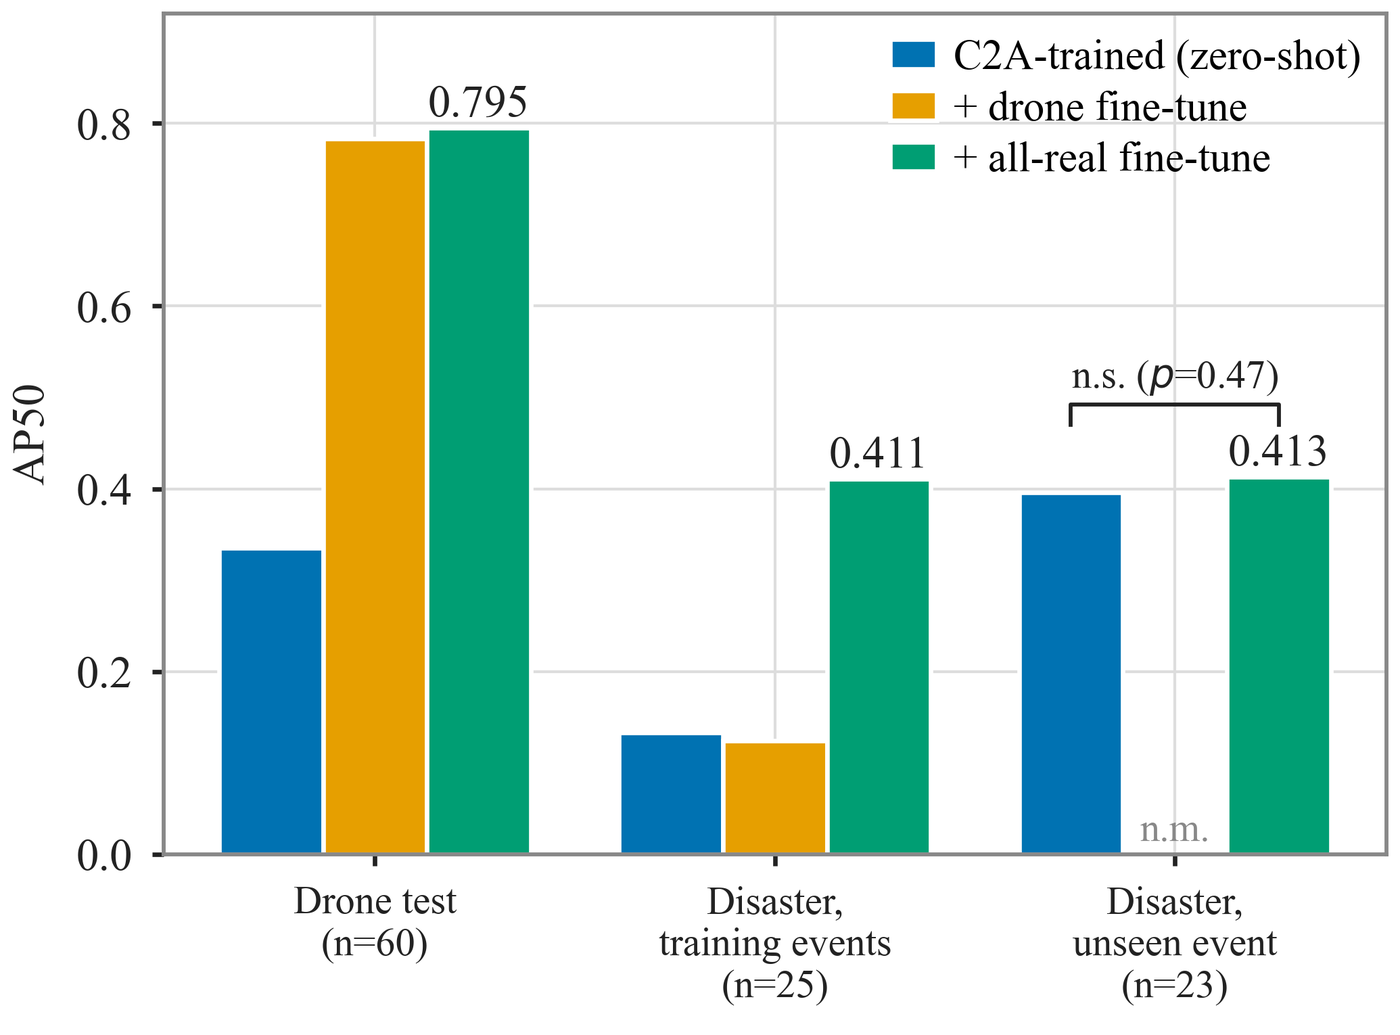
\includegraphics[width=\columnwidth]{figures/fig_adapt_stages_print.png}}
\caption{AP50 of three training stages on the three real evaluation domains.
Drone-only fine-tuning leaves disaster footage untouched (middle bars), so what
helps disaster frames is disaster labels rather than real images in general. On
an event held out from all training (right group) the adapted and base models are
statistically indistinguishable, which bounds the result.}
\label{fig:stages}
\end{figure}

\begin{table}[htbp]
\caption{The Adapted Model on Every Held-Out Set. Rec.\ is recall at the
operating threshold of 0.25.}
\label{tab:multi}
\begin{center}
\small
\begin{tabular}{|l|c|c|c|c|}
\hline
\textbf{Evaluation set} & \textbf{Images} & \textbf{AP50} & \textbf{F2} & \textbf{Rec.} \\
\hline
C2A, scene-disjoint test & 2{,}040 & 0.837 & 0.824 & 0.821 \\
\hline
Drone test & 60 & 0.795 & 0.771 & 0.837 \\
\hline
Campus & 25 & 0.689 & 0.666 & 0.718 \\
\hline
Disaster, training events & 25 & 0.411 & 0.472 & 0.451 \\
\hline
Disaster, unseen event & 23 & 0.413 & 0.451 & 0.374 \\
\hline
\end{tabular}
\end{center}
\end{table}

Three boundaries belong in the record.
\begin{itemize}
\item \textit{The adaptation is specific to the footage it saw.} On the held-out
event the adapted model scores 0.413 against the base model's 0.396, a difference
of 1.7 points whose bootstrap interval spans zero ($p = 0.47$), while precision
at the operating threshold falls by 13.1 points. Sixty frames from two events
adapt the model to those events, not to disasters in general.
\item \textit{The absolute level on real disaster imagery is modest.} At the
operating threshold the adapted model finds 482 of 1{,}070 people and roughly
half of its detections are false alarms, which suits operator-reviewed triage
rather than autonomous decisions.
\item \textit{The size regime the levers targeted is untouched on real data.}
People below 8 px in real disaster frames are not recovered at all, across all
54 such instances, by any model tested here. Every gain in
Fig.~\ref{fig:answer}(a) was measured on composited imagery, and none of it
reaches the bottom of the size range on real imagery.
\end{itemize}

\section{Conclusion}
We asked where recall of sub-8-pixel people comes from and measured four answers
on one detector. Attention is nearly free and worth 0.3 points. A stride-4
detection scale is worth a further 1.1 and is the best of the network changes,
which makes MSA-YOLO, at 0.853 AP50 and 19.6 million parameters, second among
published C2A results to a model three times its size. A bidirectional
state-space neck is worth nothing for 2.4 million parameters and 2.8 times the
latency. The assignment of supervision is worth 2.08 points at no inference cost,
more than any of them, which says that for targets this small how supervision is
assigned matters more than what is added to the network. On real footage the same
detector fell to 0.335 AP50 on drone video and 0.133 on disaster frames until 248
labeled real frames raised those to 0.795 and 0.411 at almost no cost to the
benchmark, and below 8 px it recovered nothing at all. The next gains in this
regime look more likely to come from supervision and from real data than from
further additions to the network.

\bibliographystyle{IEEEtran}
\bibliography{references}

\end{document}
